In this section, we give a detailed description of our proposed SAR approach. The overall pipeline of SAR is depicted in Figure \ref{pipeline}. Given a sketch image, the first stage in SAR is to extract major stroke contours in the image and segment these strokes into stroke segments. These strokes occur both at the silhouette and the interior of the sketch. Stroke segments from many sketches across multiple artists are grouped (using low-level image features) to form a universal dictionary of stroke segments. This dictionary is employed in a hierarchical bag-of-words model, which is used to represent a sketch image $\mathbf{I}$ as a histogram of stroke segments. We claim that this stroke histogram encodes some of the characteristics of an artist's unique style and thus can be used to discriminate this artist's sketches from others, no matter what the sketch is about. Discrimination is performed in a supervised manner using multi-class classification, where each class designates an artist. In what follows, we elaborate on the individual stages of SAR.
\vspace{-4mm}
\subsection{Stroke Extraction and Segmentation}\label{subsec: segmentation}
\vspace{-1mm}
%This section will describe stroke extraction and segmentation in detail, i.e., steps 2-3 of the SAR method.
 $\mathbf{I}$ is decomposed into strokes which are further split into stroke segments that can expose authorship. Representing sketches at such a local scale can identify stroke segments that play an essential role in authorship discrimination.
%We believe that this distinction between types of strokes will allow for a more indepth analysis of stroke authorship. It will help us determine which stroke segments in general tend to play a more important role in authorship discrimination.

%The gray value at each pixel in image $I$ is $I(i,j)\in[0,255],i=1,...,M,j=1,...,N,$ where $M$ and $N$ are height and width of the image respectively.
%\vspace{-2mm}
%\paragraph{Silhouette Extraction.} Sketch image $\mathbf{I}$ is converted to grayscale. The boundary curve of the silhouette is a set of contiguous boundary pixels ordered clockwise or anti-clockwise. We adopt the simple flood-fill method to delineate the silhouette of $\mathbf{I}$ \cite{soille2003morphological}. Since artists tend to use strong dark strokes at silhouettes, the pixels representing these silhouettes tend to have higher gradient information than their surroundings. This ensures convergence of the flood-fill method, whose intensity threshold parameter is selected adaptively using Otsu's standard thresholding method. The output of this extraction module is a tracing of the pixels on the silhouette of sketch image $\mathbf{I}$. If the silhouette is not a closed contour then this is resolved by having double silhouettes, i.e. a silhouette is traced from both sides.
%This technique searches an area of pixels with large gray values $I_u$ (light area) surrounded by pixels with small gray values $I_l$ (dark area), and vice versa. Then the light area is filled by setting its pixels to $I_l$. Thresholding is applied to connect overlapping dark areas as many as possible before filling the image. If the gray value of a pixel is smaller than the threshold, it will be set to 0 (black), otherwise, it is set to 255 (white). An empirically derived value 240 is used as the threshold. Therefore, the new image $I^t$ is: $I^t (i,j)=0$ if $I(i,j)<240$, and $I^t (i,j)=255$ if $I(i,j)\geq 240$. We use the flood fill algorithm to detect a region surrounded by 0-value pixels and its inside pixel values all equal to 255. Then every pixel in the region will be set to 0. After filling all such regions in the image, a silhouette is obtained.

\noindent\textbf{Stroke Extraction.} We use Adobe Live Trace, an off-the-shelf digitization technique, to decompose a sketch into a set of paths, each of which comprises a number of Bezier curves depicting the artistic strokes \cite{adobe123}. There exists a number of other commercial and non-commercial digitization techniques, such as the recent work by Noris et al. \shortcite{Noris:2013:TVC:2421636.2421640}. However, we choose to use Adobe Live Trace in SAR, since it stays faithful to the original sketch and it is widely accessible and easy to use. With Adobe Live trace, we can apply different levels of digitization to the original sketch and evaluate the effect of this digitization on sketch style as we discuss later in Section \ref{subsec:variations}. Extracted strokes are then traced and sampled as pixels in the image.

%It is worthwhile to note here that pixel tracing along edges has to be performed in a non-trivial manner, so as to avoid visiting the same pixels multiple times and adding redundancy to the trace.
%After that, each internal stroke is treated as an image and the silhouette stroke extraction method described above is applied to every stroke independently.


%Generally, this utility represents a sketch as a set of paths each of which has a number of Bézier curves representing the artist's strokes. We found that the resulted digitized images are visually very close to the original sketches which was the main motivation for using such utility.  After that, each internal stroke is treated as an image and the silhouette stroke extraction method described above is applied to every stroke independently.

\iffalse
%paragraph{Pixel Ordering.} Both boundary and internal strokes segmentation requires contiguous pixels for representing each stroke. Usually, a pixel loop can be connected by starting from one pixel and ending at the same pixel. Connection means that each pixel has at most two neighbors in an 8-connected neighborhood, so that pixels can be tracked one after another. The Canny operator is the most widely used method for edge extraction. However, it can result in more than two neighbors for one pixel in an 8-connected neighborhood, which leads to redundant lines. This situation is shown in Figure 2(b), in which the edges are detected by the Canny operator from Figure 2(a). To solve this problem, we use a template to search neighbors in a fixed order, along with a tag vector to avoid repeat visits.


\begin{figure}[htbp]
\centering
\subfigure[]{
  \centering
  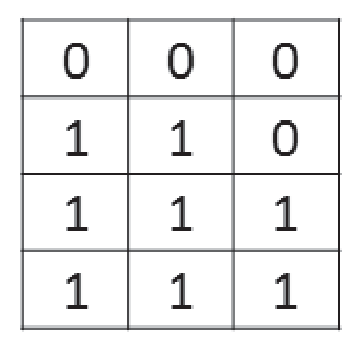
\includegraphics[width=0.1\textwidth]{images/pixOrdering1.eps}
  \label {fig:subgraph_2a}
}
\subfigure[]{
  \centering
  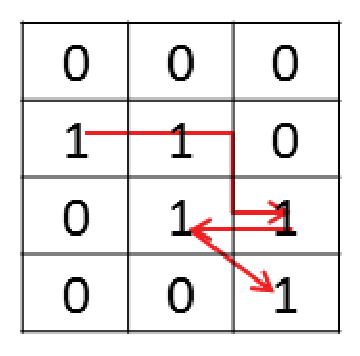
\includegraphics[width=0.1\textwidth]{images/pixOrdering2.eps}
  \label {fig:subgraph_2b}
}
\subfigure[]{
  \centering
  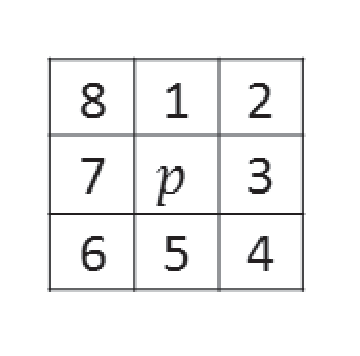
\includegraphics[width=0.1\textwidth]{images/pixOrdering3.eps}
  \label {fig:subgraph_2c}
}
\subfigure[]{
  \centering
  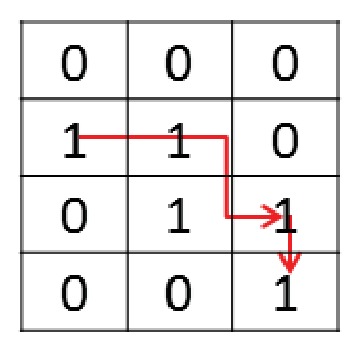
\includegraphics[width=0.1\textwidth]{images/pixOrdering4.eps}
  \label {fig:subgraph_2d}
}
\caption{Examples of edge pixels. (a) 16 pixels from the image shown in Figure2(d), where 0 is the background pixel and 1is the silhouette pixel; (b) an edge detected by the Canny operator from (a), where 1 represents edge pixels, red arrows indicate possible pixel order leading to multiple lines; (c) searching order of pixels, the middle p is the current pixel, the order of searching is labeled from 1 to 8. (d)  the revised searching order indicated by red arrows.}
\label {fig:Figure2}
\end{figure}

Let the set of edge pixels be denoted by ${P_i}, i=1,...,l$, where each pixel $P_i$ = $[P_i (x),P_i (y)]$, and $l$ is the number of pixels. The process of ordering pixels connects independent pixels ${P_i}$ according to their 8-connected neighborhood. Let the reordered pixels be placed in a $l\times2$ list $L$, where $L_1$ is the starting pixel, $L_{i+1} $is the next neighbor to $L_i$. Initially we choose an arbitrary pixel $P_k$ as the starting pixel $L_1$, set  $L_1= P_k$, and mark pixel $P_k$ as visited. Then iteratively search the next neighbor $L_{i+1}$ of $L_i$ according to the searching order given in Figure 2(c). Suppose $L_i$ is located at $p$, starting from position 1, the first unvisited $P_u$ is taken as $L_{i+1}$. The ordering process stops when the searched $L_{i+1}=L_1$. Figure 2(d) shows a revised search which avoids the polyline.
\fi


\noindent\textbf{Stroke Segmentation.} Strokes extracted from $\mathbf{I}$ can be quite long and contain a rich amount of geometric information. Modeling such a stroke as a whole entity is quite a difficult task in itself, since it should encode all possible variations that a particular stroke can take on. Instead, we resort to breaking each stroke into smaller units (called segments) that are represented in a more straightforward and conventional manner. We fit a b-spline curve to each stroke and identify break points as locations of local maximum curvature in the b-spline. We explicitly handle linear strokes by placing break points at its two ends to avoid over-segmentation. The pixels between two consecutive breakpoints (or the beginning/end of the stroke) are grouped together and denoted as a stroke segment. Figure ~\ref{fig:Figure3} shows the stroke segments extracted from two sketches taken from one of our sketch datasets.

%Figures \ref{fig:mickey} and \ref{fig:mickeyb} are examples of boundary curves with 1401 pixels and 2107 pixels from two high resolution images respectively. Curve fitting on thousands of pixels is time consuming, but high resolution images usually provide sufficient and accurate boundary and internal stroke information of the object. This is important for the SAR method because the authorship determination needs as much information as possible. To solve the time efficiency problem, we first fit a b-spline curve on pixels selected by systematic sampling from the whole pixel set $L$. Curvatures are calculated on the spline curves, and those points with local maximum curvature are selected as breaks. Then the break points will be re-located in $L$. Examples of segmentation on the boundary strokes are shown in Figure ~\ref{fig:Figure3}
\vspace{-2mm}
\begin{figure}[htbp]
\centering
\subfigure[]{
  \centering
  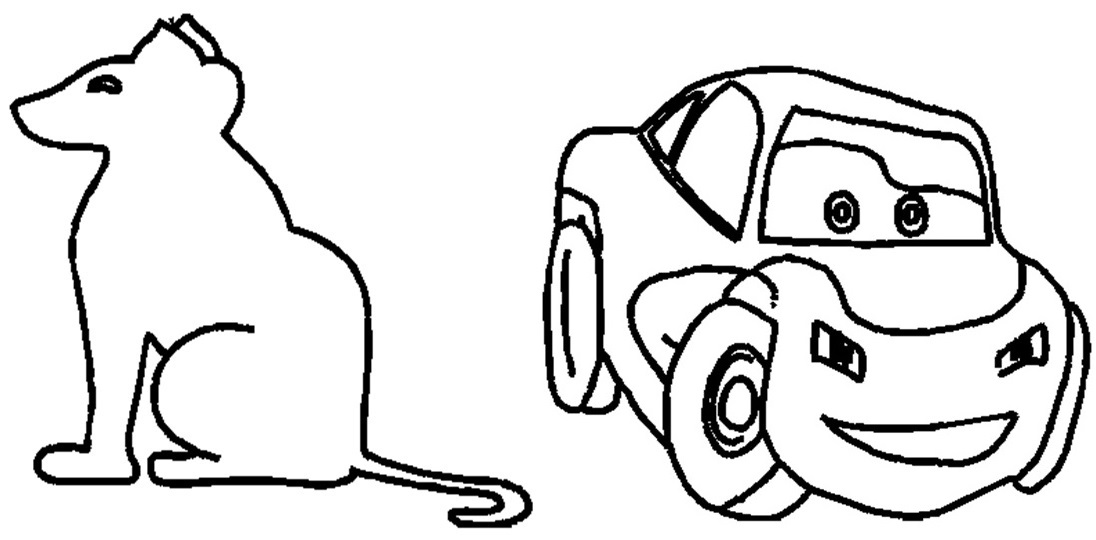
\includegraphics[width=0.21\textwidth]{images/beforeSegmantation.jpg}
  \label {fig:mickey}
}
\subfigure[]{
  \centering
  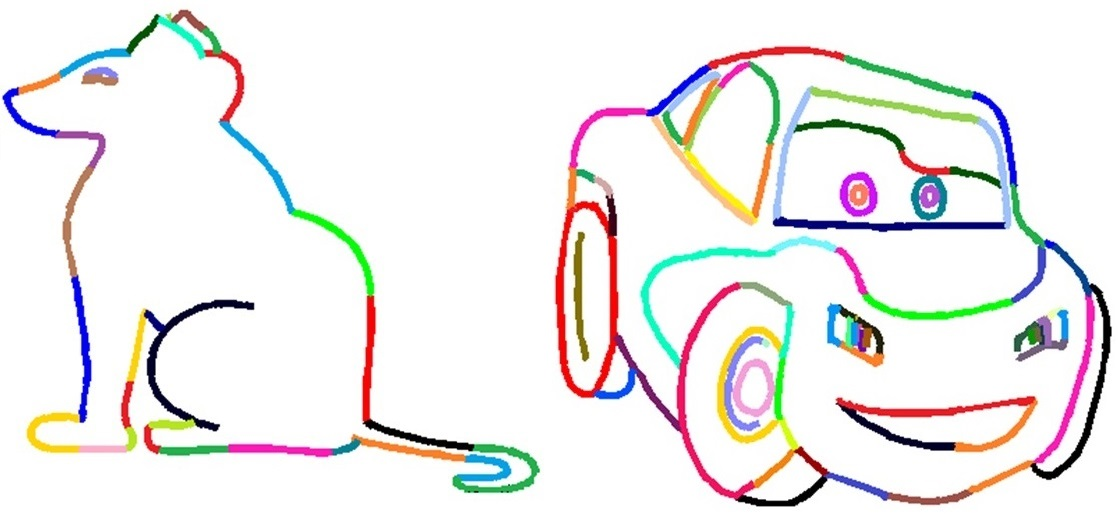
\includegraphics[width=0.21\textwidth]{images/fullSegmantation.jpg}
  \label {fig:mickeyb}
}
\vspace{-3mm}
\caption {Stroke segmentation. (a) shows two sketches after digitization and (b) shows their extracted stroke segments (color-coded)}\vspace{-3mm}
\label {fig:Figure3}
\end{figure}

% How about calling the stroke segment in this context as stroke and their union as curves or something else?

\vspace{-4mm}
\subsection{Mathematical Characterization} \label{subsec: featureExtraction}
\vspace{-1mm}
% main assumption here is that the style of an artist manifests itself in the use of particular strokes over others. We do not claim that the stroke histogram is the same across all sketches of the same artist, but we do assume that they are 'closer' to each other than to other stroke histograms. Therefore, we can find a classifier that can separate between artist sketches.
After $\mathbf{I}$ is decomposed into stroke segments, we represent it according to its stroke content.We aim to describe a stroke segment's structure and the manner in which it is drawn. We focus on local features that are simple to extract, representative, and invariant to various deformations (e.g. rotation, translation, and scale). In this paper, each segment is described by four simple features that encode eccentricity, symmetry, local consistency, and inflection. The first three features describe the stroke segment itself, while the last one describe its relationship to its neighbors. These features are both empirically validated and biologically inspired. When considering the process needed to analyze drawing traits at the stroke level, one fundamental factor arises, namely the neuro-geometry of hand-arm movement, i.e. the physiology in drawing strokes. In the foundational paper of  \cite{morasso1981spatial}, it was shown that different subjects produce hand/arm movements that are very similar to or coincide with simple curve strokes. Although low curvature change was generally maintained across different subjects and experiments, it was also found that individuals exhibited unique stroke characteristics. This finding was also confirmed in the work of  \cite{abend1982human}. In \cite{flash1985coordination}, a mathematical model based on minimizing jerk (change of curvature) and analyzing stroke velocity was verified empirically. In summary, this and other work (see references in \cite{flash1985coordination}) strongly suggest that \textbf{(1)} gesturing and strokes carry unique and identifiable aspects for an individual, and \textbf{(2)} that curvature and its change are key features for analyzing simple strokes. Inspired by the above physiological findings, we characterize stroke segments by focusing on curvature and its change in a drawn curve.

Moreover, in analyzing a large number of simple strokes, we see that a conic fit to a stroke segment is faithful to its original geometry and representative enough for the purpose of authorship recognition. From each conic, we extract eccentricity, symmetry, local consistency, and inflection features that are conveniently invariant to rigid-body deformations. Needless to say, this invariance also holds when the entire sketch is represented using stroke segment features. We give a description of these four features next.

%fit the curve’s pixels with a least squares polynomial. Among the different analytics, we looked at the evolutes of the subsequent curves (See examples, Figure. \ref{fig:evoluteofcurve}).  An evolute is the envelope of a curve’s normals. Even with high degree fits, we easily noted that evolutes of simple strokes regularly appeared to be close to the evolutes of conics as in Figure \ref{evoluteofconic}  Since conics minimize the curvature of the curve, this supported the neuro-geometry research cited above that curvature change was critical in hand/arm gestures, and it also led us to develop criteria based on 2nd order criteria, i.e. conic fits to the strokes. As an extra convenience, curvature criteria are translation, orientation and scale invariant.  This helped considerably in acquiring sample data, since information on original position, size and tilt of the drawings is not usually available for stored images.

%\SARA{Those features are both empirically derived and biologically inspired. When we considered the process needed to analyze drawing traits at the level of stroking, one fundamental factor arose is the neuro-geometry of hand-arm movement, i.e. the physiology in drawing strokes.  In the foundational paper of  \cite{morasso1981spatial} different subjects produced specified hand/arm movements that were very similar to or coincided with simple curve strokes. Although certain invariants such as low curvature change were generally maintained across different experiments, it was also found that individuals exhibited unique characteristics across a range of exercises.  The low curvature change in simple hand/arm gestures was confirmed in the thorough work of  \cite{abend1982human}, while also noting individual characteristics.  In \cite{flash1985coordination}, a mathematical model, which included stroke velocity, based on minimizing jerk (change of curvature) was verified empirically.  In total, this and other work (see references in \cite{flash1985coordination}) strongly suggest that \textbf{(1)} gesturing and strokes have unique, identifiable aspects for an individual, and \textbf{(2)} that curvature change is key for analyzing simple strokes.  We therefore characterize strokes by focusing on the individuality of curvature change in a drawn curve. Moreover, in analyzing a large variety of simple strokes, we fit the curve’s pixels with a least squares polynomial.  Among the different analytics, we looked at the evolutes of the subsequent curves (See examples, Figure. \ref{fig:evoluteofcurve}).  An evolute is the envelope of a curve’s normals. Even with high degree fits, we easily noted that evolutes of simple strokes regularly appeared to be close to the evolutes of conics as in Figure \ref{evoluteofconic}  Since conics minimize the curvature of the curve, this supported the neuro-geometry research cited above that curvature change was critical in hand/arm gestures, and it also led us to develop criteria based on 2nd order criteria, i.e. conic fits to the strokes. As an extra convenience, curvature criteria are translation, orientation and scale invariant.  This helped considerably in acquiring sample data, since information on original position, size and tilt of the drawings is not usually available for stored images.
%}

%\begin{figure}[ht]
%\centering
%\subfigure[]{
%  \centering
%  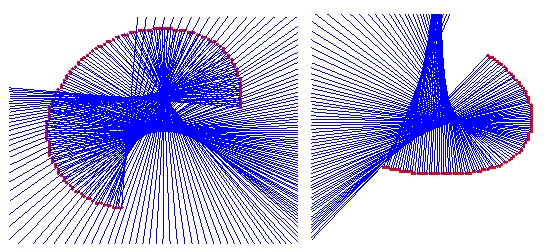
\includegraphics[width=0.26\textwidth]{images/evoluteofcurve.jpg}
%  \label {fig:evoluteofcurve}
%}
%\subfigure[]{
%  \centering
%  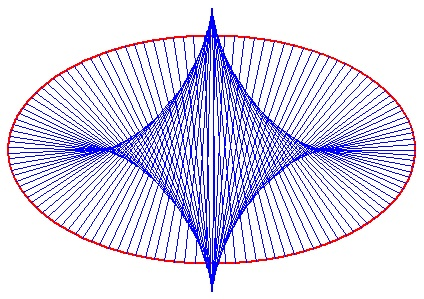
\includegraphics[width=0.18\textwidth]{images/evoluteofconic.jpg}
%  \label {fig:evoluteofconic}
%}
%\caption{(a) Evolutes of test curves (b) Evolute of a conic }
%\end{figure}
% It is worthwhile to note that other features can be used in this context, e.g. shape moments, curvature histogram, etc.

\noindent \emph{Eccentricity}: This feature represents the change of curvature in a stroke segment. It measures how the segment deviates from being circular, i.e. how rounded or sharp it is. By fitting a conic section to the stroke segment \cite{taubin1991estimation}, eccentricity ($\varepsilon$) is computed as a function of the ratio between the conic's major and minor axis lengths as in (\ref{eq: ecc}).
\vspace{-1mm}
% For example, Disney characters tend to have more rounded silhouettes using nearly elliptic curves. Compared to Disney, other cartoon companies such as Looney Tunes prefers to adorn their characters with straighter and sharper strokes.
\begin{equation}
\varepsilon=\begin{cases}
\sqrt{1-\frac{b^{2}}{a^{2}}} & \text{if the conic is an ellipse}\\
\sqrt{1+\frac{b^{2}}{a^{2}}} & \text{if the conic is a hyperbola}
\end{cases} \label{eq: ecc}
\end{equation}
\vspace{-3mm}

\noindent \emph{Symmetry}: To crudely evaluate how symmetric a stroke segment is, we simply take the absolute difference in eccentricity of the segment's two halves (refer to Figure \ref{fig:symmetry}). The segment is divided into two equal length parts (denoted as \emph{attack} and \emph{decay} following typical sketch nomenclature) and the eccentricity of each part is computed as described above.
\vspace{-2mm}

\begin{figure}[ht]
\centering
\subfigure[]{
  \centering
  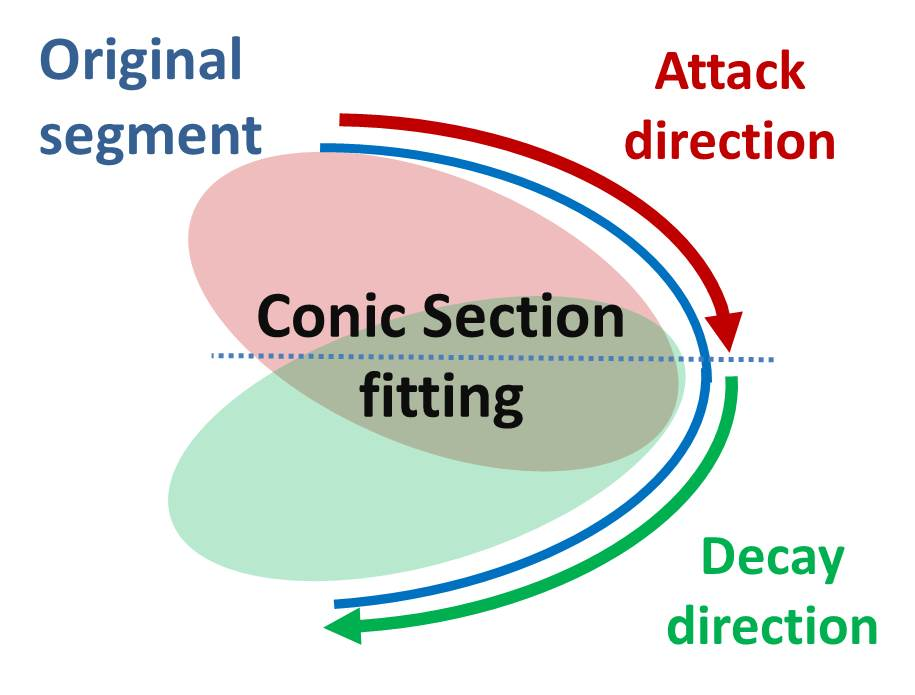
\includegraphics[width=0.18\textwidth]{images/symmetry.jpg}
  \label {fig:symmetry}
}
\subfigure[]{
  \centering
  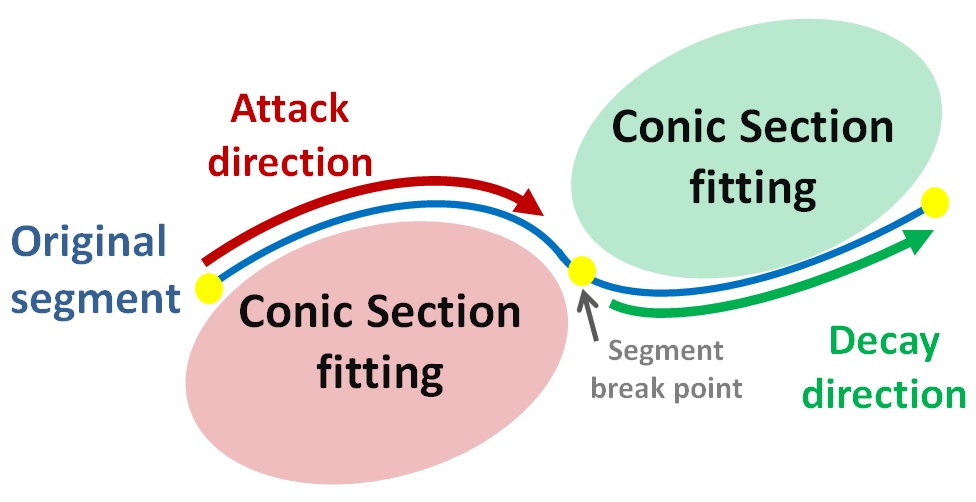
\includegraphics[width=0.26\textwidth]{images/inflection.jpg}
  \label {fig:inflection}
}\vspace{-3mm}
\caption{Attack and decay parts used to construct stroke segments. (a) shows a stroke segment divided into equal length parts enabling the computation of the symmetry feature. (b) shows two adjacent stroke segments connected by an inflection breakpoint. The inflection feature is computed by comparing these two segments.}\vspace{-6mm}
\end{figure}

\noindent \emph{Local Consistency}: This feature measures the extent of local variation within a stroke segment. It is computed as the average absolute difference between the eccentricity of the entire segment and the eccentricity of distinct overlapping parts of this segment. To generate these distinct parts, we employ a sliding window approach across the segment, where the window size is one third the size of the segment itself and the step size is half the window size. This feature captures subtle changes in shape and curvature.

\noindent \emph{Inflection}: The previous three features describe the stroke segment itself. However, characteristics of artistic style are encoded in how stroke segments are sequenced. Of special interest are locations of inflection, where the sign of curvature changes. An inflection point will be detected by SAR as a breakpoint between two stroke segments that together form a stroke (refer to Figure \ref{fig:inflection} for an example). To encode such relational information at an inflection point, we compute the absolute difference in eccentricity between each pair of stroke segments that share this inflection point. For stroke segments whose breakpoints are not inflection points, we set their inflection feature to a nominal value (-1).
%
%After we extracted a set of segments from all internal and external strokes, we fit a conic section to each curve segment. A fitted conic section can be an ellipse, parabola or hyperbola. It is an important technique in curve and surface reconstruction and has been studied thoroughly \cite{bookstein1979fitting,taubin1991estimation,zhong2007direct}. Tubin \cite{taubin1991estimation} solved the problem by minimizing the approximate mean square distance. A conic section function is given by:
%
%\begin{equation}
%Ax^2+Bxy+Cy^2+Dx+Ey+F=0,
%\end{equation}
%
%where $A$, $B$, $C$, $D$, $E$, $F$ are coefficients. The discriminant  $\Delta$, calculated by $B^2-4AC$, determines the types of conic section.  If $\Delta<0$, function (1) yields an ellipse or a circle; if $\Delta=0$, it is a parabola, and otherwise, a hyperbola. The discriminant, $\Delta$ will be set to 0 if its absolute value is less than machine epsilon 2.2204e-016 due to computation precision.
%
%Every curve segment is labeled by a specific type of conic section according to the value of $\Delta$. For different types of segments.
%
%%\noindent{\bf Local Feature Extraction.}
%After representing each curve segment with a corresponding conic section, we then calculate the eccentricity which represents the first local feature and the basis for the rest of the features. A circle has eccentricity $\varepsilon=0$, and a parabola has $\varepsilon=1$. The eccentricity of ellipse and hyperbola cannot be directly calculated by function (1). Coefficients in function (1) are converted to $(C_x, C_y, R_x, R_y, \theta)$, where $C_x$ and $C_y$ are coordinates of the center, $R_x$ and $R_y$ are the length of two axes $a$ and $b$ respectively, $\theta$ is the angle between X-axis and the major axis of the ellipse or hyperbola. Then the eccentricity $\varepsilon$ is computed by:
%\begin{equation}
%\varepsilon=\begin{cases}
%\sqrt{1-\frac{b^{2}}{a^{2}}} & \text{if} \; \Delta<0 \; (elllipse)\\
%\sqrt{1+\frac{b^{2}}{a^{2}}} & \text{if} \; \Delta>0 \; (hyperbola)\end{cases}
%\end{equation}
%
%As a general observation, using the discriminant to break down the quadratic fitting adds additional information to the process. Eccentricity reflects to what extent a conic section deviates from being circular so that the analysis of its distribution is representative of characteristics on the strokes of a shape.

%Another two local features are based on calculating the difference in eccentricity values between what we call the attack and decay parts of an artist's stroke which represent the first and the second halves of a given stroke respectively. In other words, we examine how symmetrical an artist's stroke is. The first feature of this type is applied at shoulder shaped strokes, i.e. between two break points of a segment as shown in ~\ref{fig:symmetry}. The second feature, on the other hand, is applied between the two sides of an inflection point as shown in ~\ref{fig:inflection}. The fourth and last local feature we extracted is based on comparing the difference in eccentricity values between global and local curves where global curves are the actual curve segments and local curves are portions of the global curves. We divide each global curve into 3 local curves and find the differences in eccentricity values between the local curves in comparison with the global one. {\color{red}[Mention that these features are rotation, translation, and scale invariant.][Other descriptive features (e.g. ) can be used to represent a stroke segment.]}

\vspace{-4mm}
\subsection{Feature Frequency Distribution} \label{subsec: featureExtraction}
Having each stroke segment $s_i$ of sketch image $\mathbf{I}$ characterized by the 4D feature vector of the features described above,
this stage represent $\mathbf{I}$ as distribution of frequency of those features.


\noindent\textbf{Building a Universal Stroke Segment Dictionary.} Our assumption is that the frequency in which an artist uses particular types of strokes is a suitable indicator of his/her authorship. To formalize this observation, we compile a dictionary of stroke segments that tends to be universal among different artists. The dictionary is learned on the stroke segments of the sketches that are used in training only. To construct a dictionary of $n$ elements, we apply hierarchical k-means clustering on a large set of stroke segments. In our experiments, we set $n=60$. We denote this dictionary as the universal stroke segment dictionary as it tends to capture the most commonly used stroke segments among artists. This clustering step is first stage of the bag-of-words (BoW) model that is popularly used to represent natural images for image classification \cite{Sivic03}. We use hierarchical k-means, since it is more robust and less sensitive to the choice of $n$ than traditional k-means clustering. And it generates a tree of $n$ cluster centers (and not only a set of centers as in the case of k-means), which encodes the membership of any stroke segment at all levels of the tree and not just the leaves. To encode a stroke segment, one has to \emph{traverse} this tree starting from the root and recursively select among its children the nearest cluster center in 4D feature space. As a result, each stroke segment is encoded as a binary membership vector of length $n$, where each value reflects whether the feature traversed the corresponding tree node or not. In Figure ~\ref{fig:bagOfWords}, we show image examples of cluster centers in the universal stroke segment dictionary, as well as, the color-coded membership of each stroke segment in a sketch. Such assignment is independent of where a stroke segment exists in a sketch.


%After extracting all the local features from all the sketches, we build a visual vocabulary and for that we use a hierarchical version of k-means clustering. K-means clustering is recursively applied to compute finer and finer partitions which returns a tree where each node is a cluster center that is used to build the visual vocabulary. We choose hierarchical k-means clustering because it gave us a better visual vocabulary representation when compared against k-means clustering and visual words of regular interval values. Figure ~\ref{fig:bagOfWords} shows a sample of strokes from the dictionary of visual words along with its color coding representation on one of the sketch's silhouette.
\vspace{-4mm}
\begin{figure}[ht]
\centering
\subfigure[]{
  \centering
  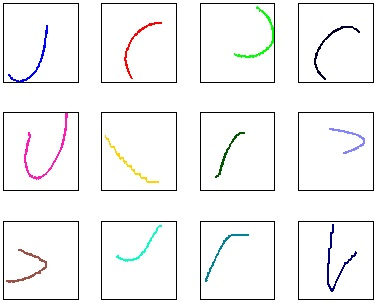
\includegraphics[width=0.24\textwidth]{images/bow.jpg}
  \label {fig:BoW}
}
\subfigure[]{
  \centering
  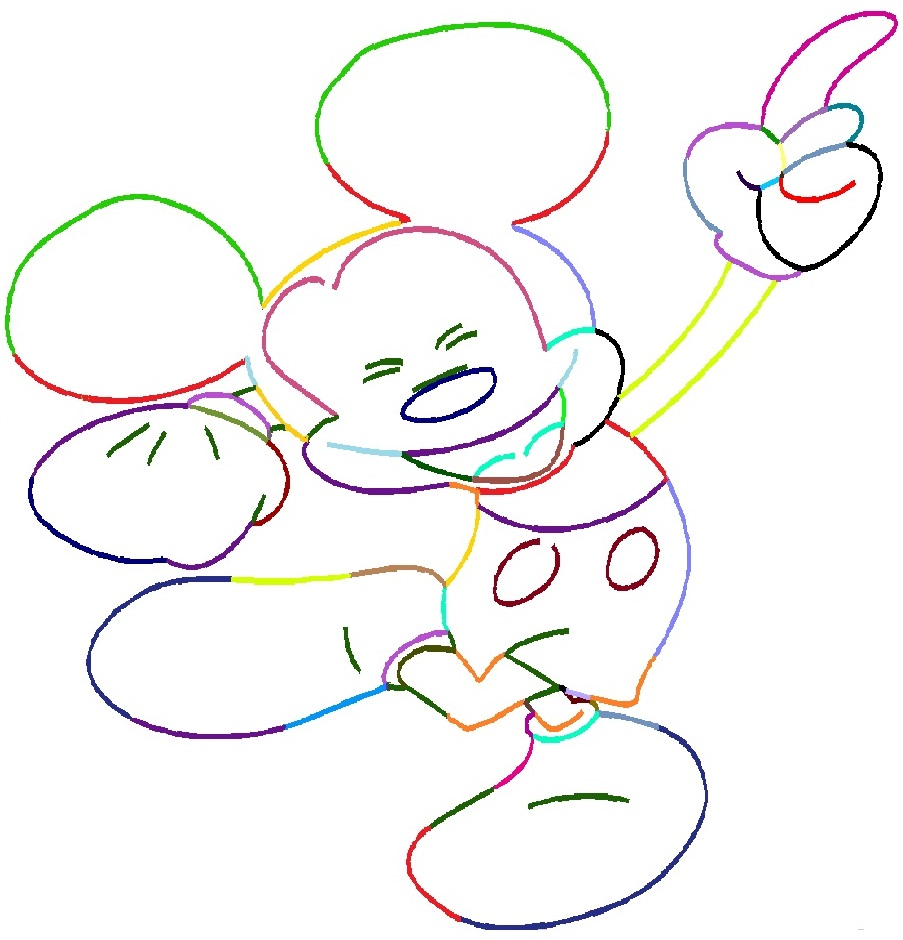
\includegraphics[width=0.20\textwidth]{images/MickyCenters.jpg}
  \label {fig:BoWSketch}
}\vspace{-3mm}
\caption{(a) Some elements of the universal stroke segment dictionary constructed from the segments of the training sketches. (b) Color-coded nearest neighbor assignment of segments to dictionary elements.}\vspace{-2mm}
\label{fig:bagOfWords}
\end{figure}

%\vspace{-2mm}
\noindent\textbf{Bag-of-Words Features.} After constructing the universal dictionary, we represent a sketch as a histogram of stroke segments following the traditional Bag-of-Words (BoW) framework. Sketch image $\mathbf{I}$ containing $m$ stroke segments produces $m$ binary membership vectors each of length $n$. These membership vectors are pooled together to produce the BoW feature vector $\mathbf{f}_{\mathbf{I}}$. We use Gaussian weighted mean pooling to encode the frequency in which an artist uses each element of the universal dictionary. As we will see, coupling $\mathbf{f}_{\mathbf{I}}$ with a discriminative model enables authorship recognition. Since the original 4 stroke segment features are invariant to rotation, translation, and scale, the BoW feature vector is invariant to these deformations \cite{lu2007survey}.


 %our bag of visual words, we use a normalized frequency histogram of visual words to represent each sketch. We apply what is called 'hard' assignment of locally extracted features to visual words \cite{Sivic03}. Such representation is what going to be used during authorship classification.

%Since the style of an artist manifests itself in the artist's use of particular stroke segments over others, representing $\mathbf{I}$

\vspace{-3mm}
\subsection{Authorship Recognition}
\vspace{-1mm}
So far, a sketch image is represented by a sparse $n$-dimensional histogram depicting the frequency in which each type of stroke segment is used by the artist in the sketch. As such, we expect the BoW feature to possess enough discriminative power to determine authorship based on simple strokes alone. We validate this assumption empirically in Section \ref{subsec:recognition}. Given a training set of sketches labelled according to the artist who drew them, we build a discriminative model using the training BoW features. In order to reduce testing time and to pinpoint the most discriminative portions of the BoW feature, we employ a forward feature selection procedure, which greedily appends a single feature at a time \emph{only} if this addition improves classification accuracy \cite{574797}. Based on our experiments, only a small subset of the $n$ features is actually used for discrimination. Using these subsampled BoW histograms, we build a multi-class classifier to assign authorship to an unseen sketch image. For sketch fraud detection, we use a binary classifier (original vs. fraudulent) instead. We experimented with a variety of classifiers and found that either an RBF (Radial Basis Function) kernel SVM or a kNN classifier can be used for this purpose. However, we decided on the kNN classifier because of its better generalizability properties and its minimal training time. We use two experimental setups to evaluate the accuracy of our classifier: 2-fold cross validation and leave-one-out. The first is a popular setup in image classification, while the latter sheds light on how dependent the classifier performance is to the amount of training data.

%\noindent{\bf Attribute Selection.}
%After Extracting all the local features all segments of a sketch, We implement a simple attribute filtering algorithm. Shall I write about this in details?

%The fourth step of SAR is to use curve features to recognize figures' authorships and classify them accordingly. Classification models are built in the new feature space, i.e. histograms of visual words. SVM and k-NN are used for categorizing objects by their authorships.

%We use nearest-neighbor classification. We find the $k$ nearest neighbors (knn) for a given histogram representation of a sketch. A histogram will belong to the category where most of the k nearest neighbors belong to. We use leave-one our and 5 fold cross validation in our experiments.
